\documentclass[12pt, a4paper]{article}
\usepackage[utf8]{inputenc}
\usepackage{footnote}
\usepackage{hyperref}
\usepackage{fullpage}
\usepackage{amsmath}
\usepackage{multicol}
\usepackage{amsfonts}
\usepackage{pgfplots}
\usepackage{pgfplotstable}
\pgfplotsset{compat=1.8}
\usepackage{cleveref}
\usepackage{graphicx}
\usepackage{tocbibind}
\DeclareMathOperator*{\argmin}{\arg\!\min}
\newcommand{\colvec}[1]{\ensuremath{\begin{pmatrix}#1\end{pmatrix}}}

\begin{document}
\title{Bachelorarbeit\\ zur Erlangung des akademischen Grades\\ Bachelor of Science}
\author{Zachary Schellin\\376930}
\noindent
\maketitle
\newpage
\tableofcontents
\newpage
\section{Introduction}
The Bhatnagar, Gross, Krook equation (BGK) is a kinetic collision model of ionized and neutral gases valid for rarefied as well as other pressure regimes \cite{BGK}. Generating data of such a flow field is essential for various industry and scientific applications[\textbf{REF}]. With the intention to reduce time and cost during the data generating process, experiments were substituted with computational fluid dynamics (CFD) computations. Consequently reduced-order models (ROMs) coupled to aforementioned computations were introduced to further the reduction of time and cost. The thriving field of artificial intelligence operates in model order reduction for data visualization/analysis since the 80's (Quelle?)  and has now surfaced in fluid mechanics. This thesis will cover the use of artificial intelligence for model order reduction in fluid mechanics.
\subsection{State of the art}
State of the art model reduction of dynamical systems is done via proper orthogonal decomposition (POD) which is an algorithm feeding on the idea of singular value decomposition (SVD)\cite{Franz}\cite{Kutz}. POD captures a low-rank representation on a linear manifold. So called POD modes, derived from SVD, describe the principle components of a problem which can be coupled within a Galerkin framework to produce an approximation of lower rank. 
\begin{equation}
	f(x)\approx \tilde{f}(x) \qquad\ \textrm{with}\qquad rk(f(x)) \gg rk(\tilde{f}(x))
\end{equation}
Bernard et al. use POD-Galerkin with an additional population of their snapshot database via optimal transport for the proposed BGK equation, bisecting computational run time (cost) in conjunction with an approximation error of ~ 1 \% \cite{Bernard}. Artificial intelligence in the form of autoencoders replacing the POD within a Galerkin framework is evaluated against the POD performance by Kookjin et al. for advection-dominated problems\cite{Carlberg} resulting in sub 0.1\% errors. An additional time inter- and extrapolation is evaluated. Using machine learning/ deep learning for reduced order modeling in CFD is a novel approach although "the idea of autoencoders has been part of the historical landscape of neural networks for decades"\cite[p.493]{Goodfellow}. Autoencoders, or more precisely learning internal representations by the delta rule (backpropagation) and the use of hidden units in a feed forward neural network architecture, premiered by Rumelhart et al. (1986) \cite{Rumelhart}.  Through so called hierarchical training Ballard et al.(1987) introduce a strategy to train auto autoassociative networks (nowadays referred to as autoencoders), in a reasonable time promoting further development despite computational limitations \cite{Ballard}. The so called bottleneck of autoencoders yields a non-smooth and entangled representation thus beeing uninterpretable by practitioners\cite{Rifai2011} leading to developements in this field. Rifai et al. introduce the contractive autoencoder (CAE) for classification tasks (2011), with the aim to extract robust features which are insensitive to input variations orthogonal to the low-dimensional non-linear manifold by adding a penalty on the frobenius norm of the instrinsic variables with respect to the input, surpassing other classification algorithms \cite{Rifai2011}. Subsequent development emerges with the manifold tangent classifier (MTC) \cite{Rifai_2011a}. A local chart for each datapoint is obtained hence characterizing the manifold  which in turn improves classification performance. On that basis a generative process for the CAE is developed. Through movements along the manifold with directions defined by the Jacobian of the bottleneck layer with respect to the input \begin{math}	\vec{x}_m=JJ^T \end{math}, sampling is realized \cite{rifai2012generative}. 
\subsection{Objective of this thesis}
Due to the non-linearity of transport problems in particular shock fronts, the construction of a robust ROM for those cases poses several challenges. Proper orthogonal decomposition (POD) and it's numerous variants like shifted-POD\cite{bibid}, POD-Galerkin\cite{bibid}, POD+I \cite{bibid} to name only a few of them, try to solve this problem by......
\subsection{Thesis outline}
\section{The BGK Equation}
The Knudsen number \cref{knudsen} introduced by Danish physicist Martin Knudsen is a measure for the rarefaction of gases. In \cref{knudsen} $\lambda$ represents the mean free path and L the characteristic length \cite{Bernard} of a particle. The mean free path  describes the average distance a particle may travel between successive impacts [\textbf{WIKI}]. For idealized gases the mean free path can be calculated via \cref{lambda}. In \cref{lambda} $k_b$ is the Boltzman constant, p is the total pressure, T is the thermodynamic temperature and d is the hard shell diameter [\textbf{WIKI}]. 
\begin{multicols}{2}
	\begin{equation}
		Kn = \frac{\lambda}{L}
		\label{knudsen}
	\end{equation}
	\begin{equation}
		\lambda = \frac{k_bT}{\sqrt{2}\pi d^2p}
		\label{lambda}
	\end{equation}
\end{multicols}\noindent
For Kndusen numbers $Kn > 10^·{-2}$ collisions are predominant in comparison to free transport, whereas for $Kn < 10{-2}$ free transport becomes the predominant behavior compared to collision\cite{Bernard}. This difference in turn characterizes flows where the Bolzmann equation (collisions) or the Navier-Stokes equations (free transport) are valid. Hence the former \cref{Boltzmann} describes the dynamics of a gas flow, where f is the probability density distribution function for a particle at point $\textbf{x} \in \mathbb{R}^3$ with velocity $\xi \in \mathbb{R}^3$ at time $t \in \mathbb{R}$. 
\begin{equation}
	\partial_t f(\textbf{x}, \xi, t) + \xi \Delta_x f(\textbf{x},\xi,t) = Q(f,f)
	\label{Boltzmann}
\end{equation}
Originally Q is often the binary Boltzmann collision term, which can be intractable in pratice \cite{BGK}. Thus the BGK equation utilizes the BGK-Operator for the collision term Q(f,f) \cref{Collision}\cite{Bernard}.
\begin{align}
Q(f,f) &= \frac{M_f(\textbf{x},\xi,t) - f(\textbf{x},\xi,t)}{\tau(\textbf{x},t)} \label{Collision}\\
M_f(\textbf{x},\xi,t) &= \frac{\rho(\textbf{x},t)}{(2\pi T(\textbf{x},t))^{\frac{3}{2}}}\exp(-\frac{||\xi -U(\textbf{x},t)||^2}{2T(\textbf{x},t)})  \label{Maxwellian}\\
\tau(\textbf{x,t}) &= \frac{Kn}{\rho(\textbf{x},t)T^{1-\nu}(\textbf{x},t)} \label{Relaxation}
\end{align}
For many kinetic gas problems it is sufficient to replace the complexity of the Boltzmann collision term by a mean-free-path approach. $\tau$ is referred to as the relaxation time, considering the fact, that collisions tend to relax the distribution function to an equilibrium state $f_0$, where $f_0 = M_f$ the equilibrium state is approximated by a Maxwellian distribution function\cite{BGK}. In \cref{Maxwellian} $U(\textbf{x},t) = (u(\textbf{x},t),v(\textbf{x},t),w(\textbf{x},t))^T$ is the macroscopic velovity, $T(\textbf{x},t) \in \mathbb{R}$ and $\rho(\textbf{x},t)\in \mathbb{R}$is the temperature and density of the gas respectively. In \cref{Relaxation} $\nu\in\mathbb{R}$ is the exponent of the viscosity law of the gas. As a result one obtains th BGK equation which can be utilized for both hydrodynamic and rarefied regimes and meets global conservation as discussed in \cref{FeaturesSOD}. By multiplying the BGK equation with the collision invariants $\Phi(v) = (1,\xi,\frac{1}{2}\xi^2)^T$ and integrating over velocity space $d\xi$, one obtains the corrsponsing moments, \cref{moment1} to \cref{moment3}.
\begin{multicols}{3}
	\begin{equation}
		\rho(x,t) = \int f d\xi \label{moment1}
	\end{equation}
	\begin{equation}
		\rho u(x,t) = \int \xi f d\xi \label{moment2}
	\end{equation}
	\begin{equation}
		E(x,t) = \int \frac{1}{2}\xi^2 f d\xi \label{moment3}
	\end{equation}
\end{multicols}
\subsection{Macroscopic features of Hydrodynamic and Rarefied Gas Flows in the SOD-Shock Tube} \label{FeaturesSOD}
\begin{figure}[!htbp]
	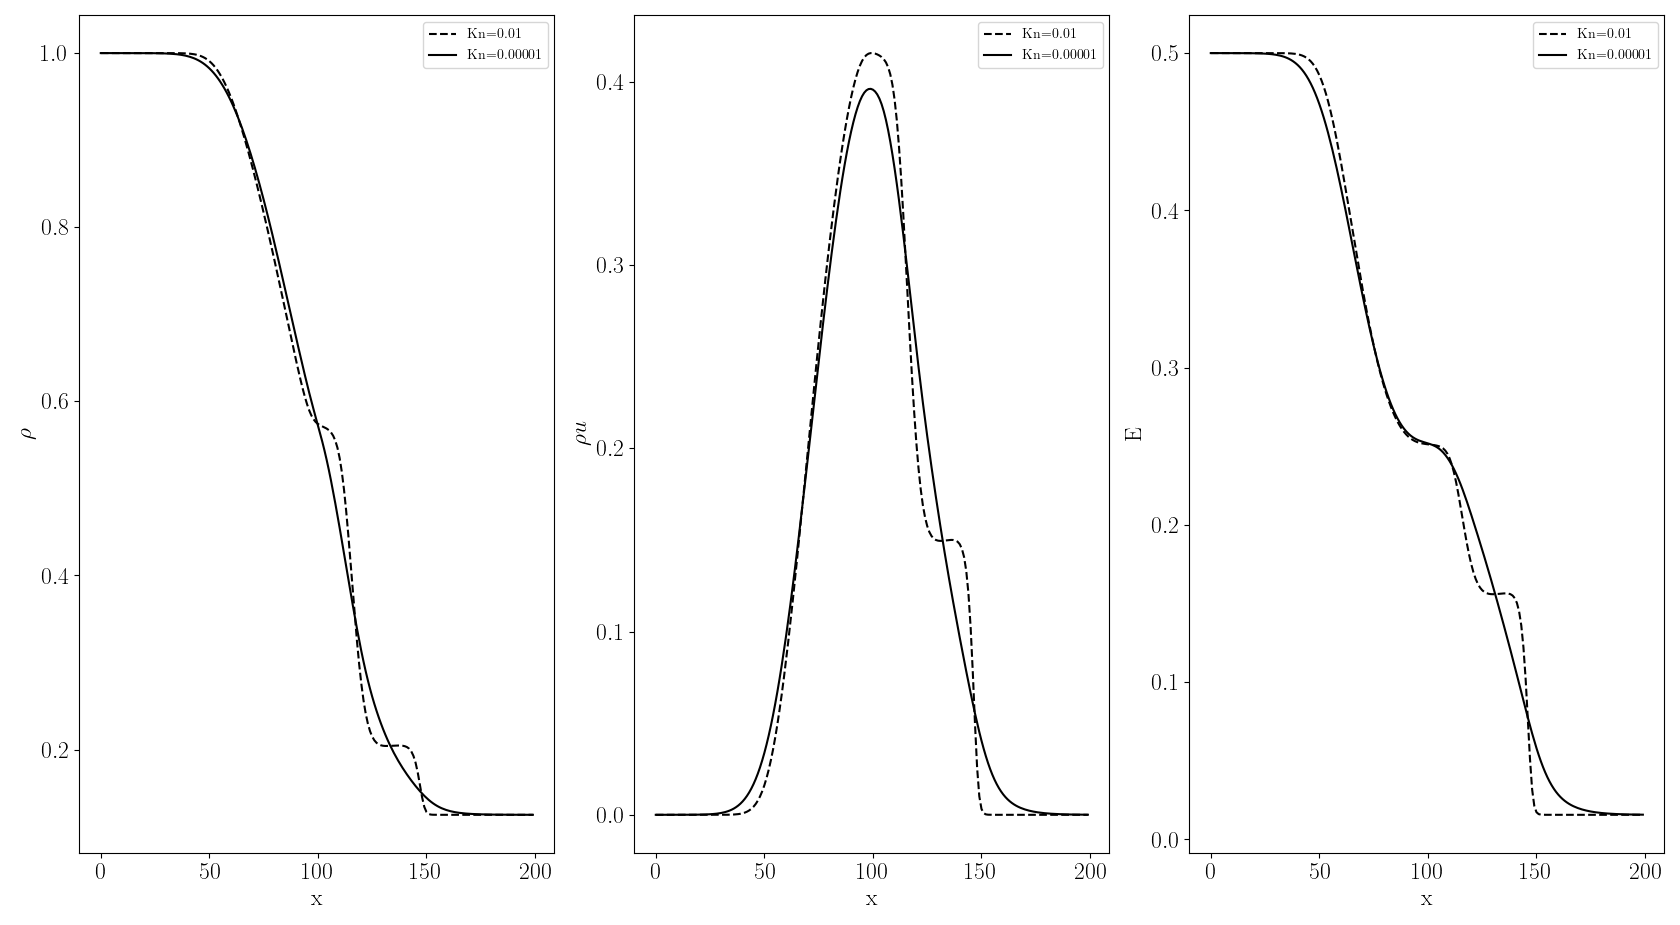
\includegraphics[width=\textwidth]{Figures/Macroscopic_Quantities_Original.png}
\end{figure}
\section{Reduced Order Algorithms}
\subsection{Data Sampling}
For the autencoder using fully connected layers, the input vectors $y_o \in \mathbb{R}$ of size $n_{input} = n_{\xi} = 40$ are arranged in the sampling matrix $S_{AE} \in \mathbb{R}^{5000x40}$ as seen in \cref{AE_matrix} resulting in $n_S = 5000$ available samples. Note that the POD uses the same matrix transposed $S_{AE}^T$ as input.
\begin{multicols}{2}
		\begin{equation}
		S_{AE} = \begin{bmatrix}
		f(\xi_1,t_1,x_1)&\cdots &f(\xi_n,t_1,x_1) \\
		f(\xi_1,t_1,x_2)&\cdots &f(\xi_n,t_1,x_2) \\
		\vdots& \vdots & \vdots\\
		f(\xi_1,t_1,x_n)&\cdots &f(\xi_n,t_1,x_n)\\
		f(\xi_1,t_2,x_1)&\cdots &f(\xi_n,t_2,x_1)\\
		\vdots & \vdots & \vdots\\
		f(\xi_1,t_n,x_n)&\cdots &f(\xi_n,t_n,x_n)
		\end{bmatrix}
		\label{AE_matrix}
		\end{equation}\break
		\begin{equation}
		S_{Conv}= \begin{bmatrix}
		n_{Filters}&f(\xi_1,\textbf{t},\textbf{x})\\
		n_{Filters}&f(\xi_2,\textbf{t},\textbf{x})\\
		\vdots\\
		n_{Filters}&f(\xi_n,\textbf{t},\textbf{x})
		\end{bmatrix}
		\label{Conv_matrix}
		\end{equation}
\end{multicols}\noindent
Convolutional autoencoders use a different sampling matrix $S_{Conv}$ due to their two dimensional capability resulting in $n_S = 40$ available samples \cref{Conv_matrix}.$N_{Filters}$ varies over the succeeding layers, growing with the shrinkage of $(\textbf{t},\textbf{x})$.
\subsection{POD}
The singular value decomposition of the input $X$ [REF to Section 1] gives the optimal low-rank approximation $\tilde{X}$ of $X$ \cref{Eg:eckard-young}[Eckard-Young]. \Cref{Fig:cumu_sing} shows the singular values (left) and the cumulative energy (right) derived from \cref{Eq:cumsum}:
\begin{equation}
S_N = \sum_{k=1}^{N}a_k \qquad\textrm{with a sequence} \qquad\{a_k\}_{k=1}^{n} 
\label{Eq:cumsum}
\end{equation}
\begin{equation}
\underset{\tilde{X}, s.t. rank(\tilde{X})=r}{\operatorname{argmin}} || X -\tilde{X} ||_F=\tilde{U}\tilde{\Sigma}\tilde{V}^*
\label{Eg:eckard-young}
\end{equation}
\subsection{Autoencoders}
\subsection{Architectures}
\subsubsection{Fully Connected}\label{Fully Connected}
The autoencoder architecture 1.0 is a composition of five fully connected layers, \cref{f_AE}. The subscript F denotes fully connected layers opposed to the subscript C which denotes convolutional layers in \cref{Convolutional}.
\begin{equation}
	y_p = f_{F}^5(f_{F}^4(f_{F}^3(f_{F}^2(f_{F}^1(y_o)))))
	\label{f_AE}
\end{equation}
Two input/output layers of size $n_{input}=40$, two hidden layers of size $n_{hidden} = 20$ and one "bottleneck" layer of size $n_{code} = 3$. The trainingloss is the mean-squared error (MSE) between the input and output of the autoencoder, where $y_0$ is the original inpput vector and $y_p$ is the reconstructed output vector \cref{MSE}.
\begin{equation}
	MSE = \frac{(y_p - y_o)^2}{n_{batch}}
	\label{MSE}
\end{equation}
\subsubsection{Convolutional}\label{Convolutional}
The convolutional autoencoder architecture 1.1 is a composition of six convolutional and three fully conected layers, \cref{f_Conv}.
\begin{equation}
y_p = f_{C}^9(f_{C}^8(f_{C}^7(f_{F}^6(f_{F}^5(f_{F}^4(f_{C}^3(f_{C}^2(f_{C}^1(y_0)))))))))
\label{f_Conv}
\end{equation}
\subsubsection{Training}
During training every 1000 epochs a sample against its prediction was printed in order to link the value of the L1-Loss to a prediction. Using this method a first verification of the model was achieved. Continuing the search for any possible shortage of the models performance, that this method could not cover, eg. samples lying between every 1000 sample, that the model was not able to reconstruct correctly, a second verification process is conducted.
\subsection{Reducd Order Model} 
\section{Results and Latent Manifold Properties}
\subsection{Evaluation Methods}
\subsection{Results}
\subsubsection{POD}
The first five singular values give an accurate approximation $\tilde{X}$ of $X$.  
As a means to evaluate the low-rank approximation of $X$ we will compare the density derived from \cref{Eq:dense}, computed from $X$ and $\tilde{X}$.
\begin{figure}[htbp!]
	\centering
	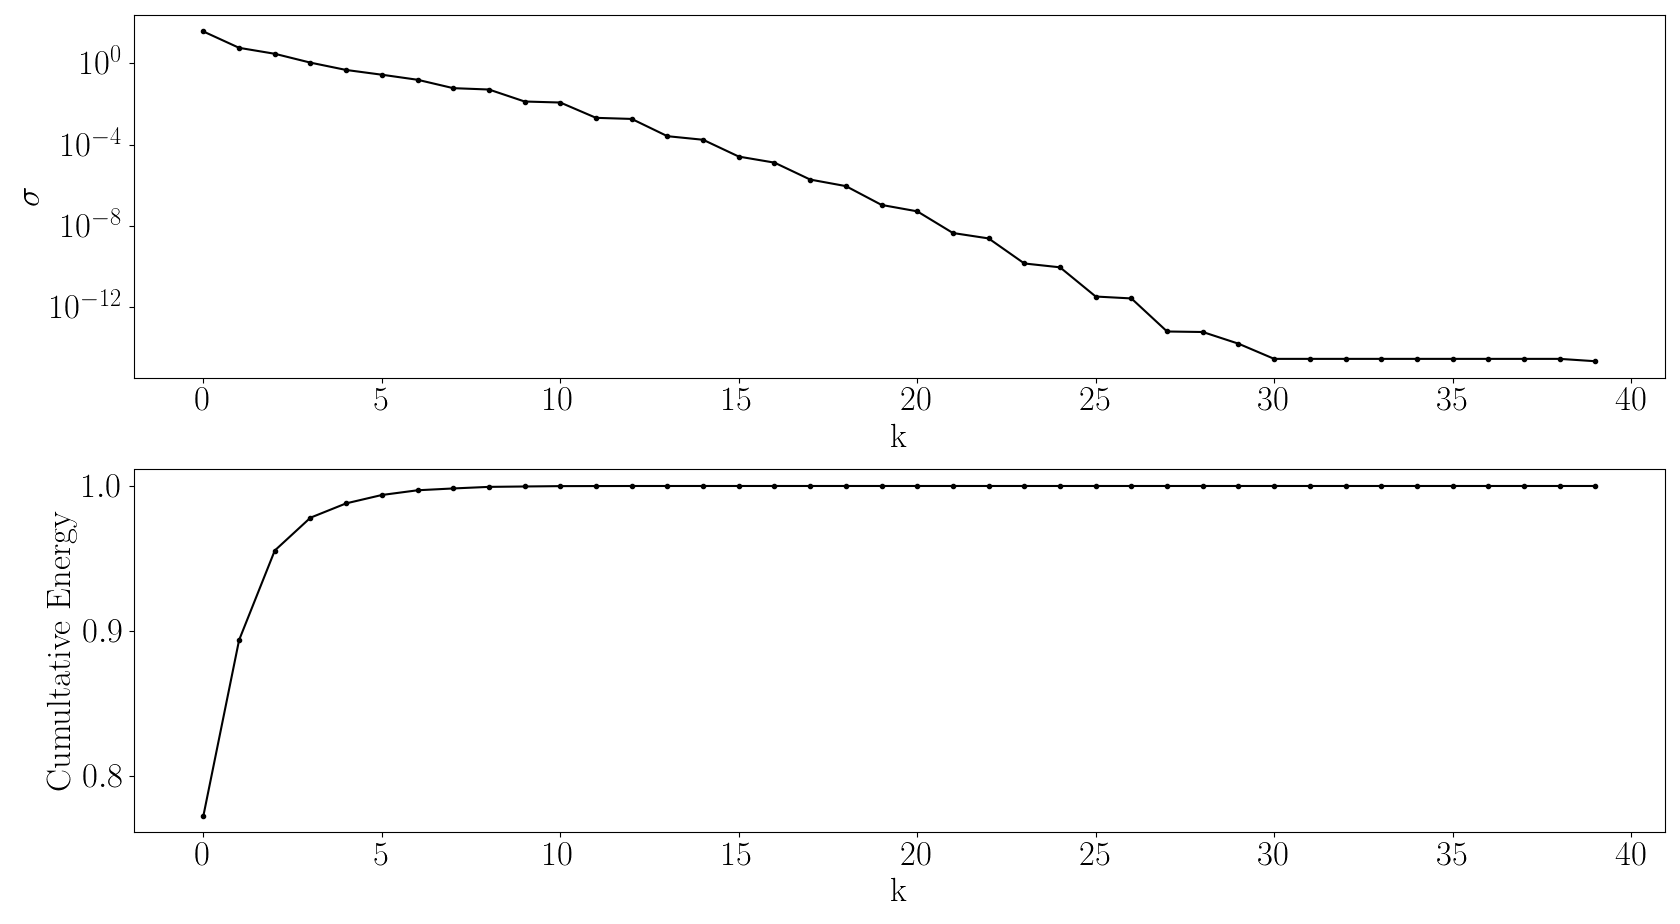
\includegraphics[width=\textwidth]{Figures/Cumultative_Singular_Values_kn001.png}
	\caption{Singular Values (left) and cumultative enrgy (right) over the number of singular values}
	\label{Fig:cumu_sing}
\end{figure}
\subsubsection{Fully-Connected Autoencoder}

The search for a reduced model of the BGK equation yields a first reduction and analysis of the provided data with a low Knudsen number of $Kn = 0.00001$. For this flow field the Navier Stokes equations are still valid.
Analysing the batch size for the architecture 1.0 the test errors in \cref{Tab:Batch} can be produced.
\begin{table}[!htbp]\centering
	\begin{tabular}{ |c c| }
		\hline
		Architecture & 1.0  \\ [.5ex]
		\hline
		Batch Size & L2-Error \\ \hline
		64 & 0.008  \\ 
		32 & 0.0049\\ \hline
		16 & 0.0038\\ \hline
		8 & 0.0037\\ \hline
		4 & 0.0026\\ \hline
		2 & 0.0021\\
		\hline
	\end{tabular}
	\caption{L2-Error over Batch-Size}
	\label{Tab:Batch}
\end{table}
For the evaluation of the prediction the Autoencoder produces normalized conservative quantities are analysed. The conservative quantities are the total energy E, the density $\rho$ and the impulse $\rho u$. Normalization is done over the temporal mean as seen in \cref{Eq:Con1} to \cref{Eq:Con3}.
\begin{figure}[!htbp]
	\minipage{0.32\textwidth}
	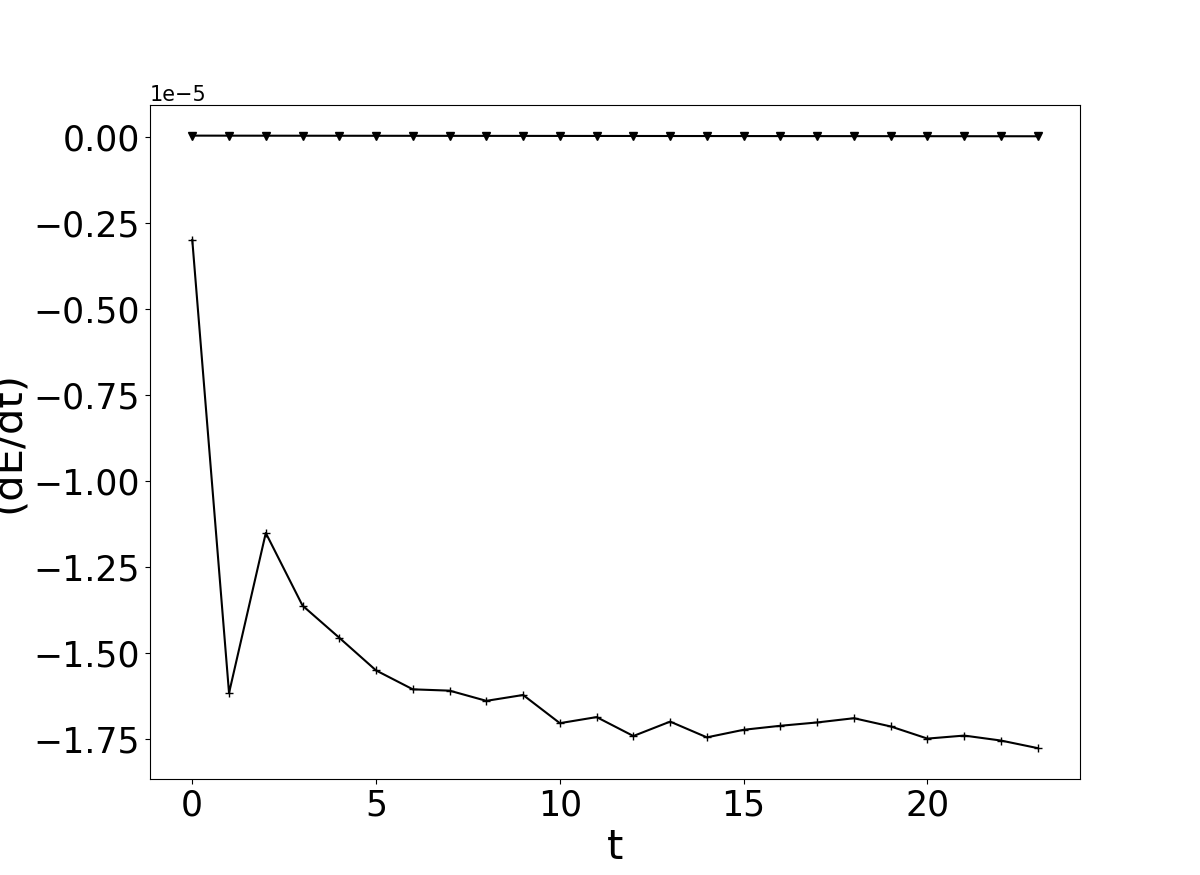
\includegraphics[width=\linewidth]{/home/zachi/Documents/ROM_using_Autoencoders/Bachelorarbeit/Figures/02_12_20/kn0p00001Conservative_Quantities/together/d_dt_E.png}
	\caption{Normalized total change in Energy $\hat{E}$ over time }\label{fig:awesome_image1}
	\endminipage\hfill
	\minipage{0.32\textwidth}
	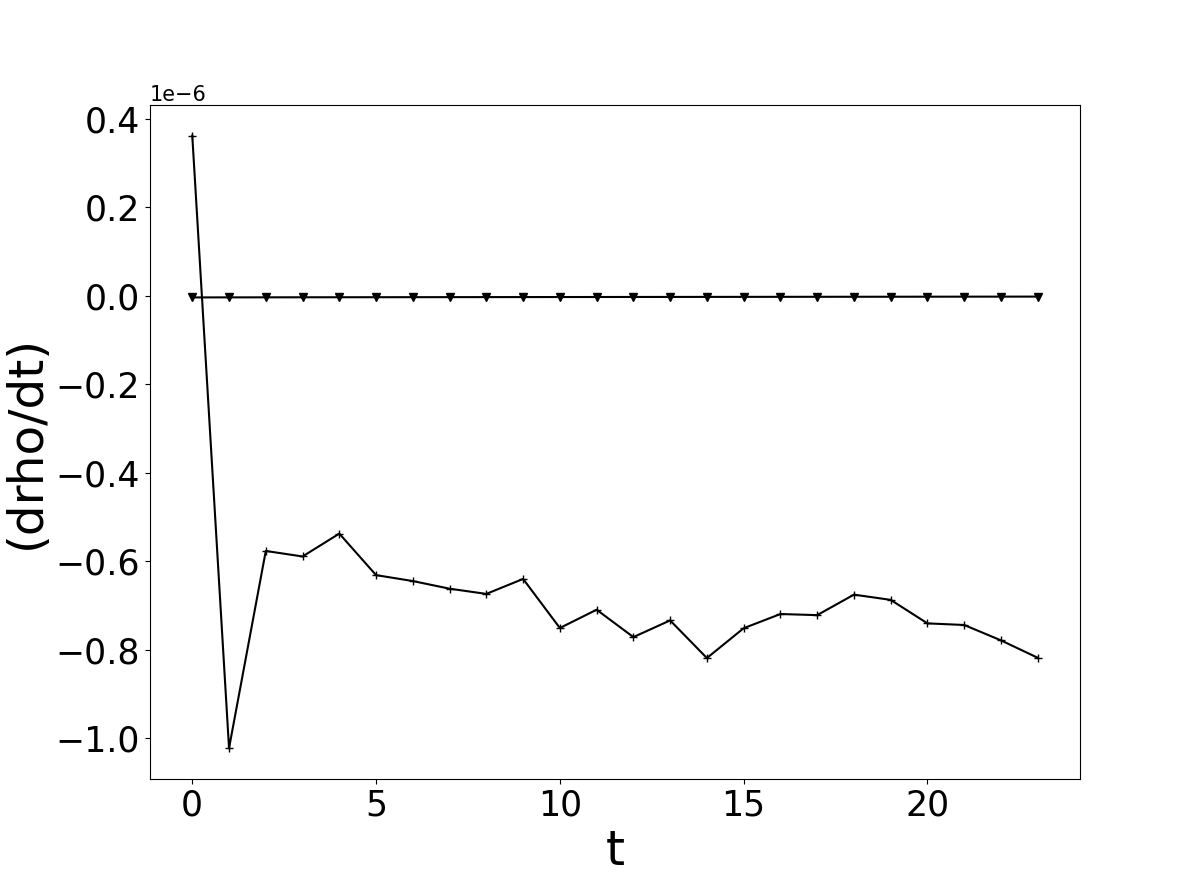
\includegraphics[width=\linewidth]{/home/zachi/Documents/ROM_using_Autoencoders/Bachelorarbeit/Figures/02_12_20/kn0p00001Conservative_Quantities/together/d_dt_rho.png}
	\caption{ormalized total change in Energy $\hat{\rho}$ over time}\label{fig:awesome_image2}
	\endminipage\hfill
	\minipage{0.32\textwidth}%
	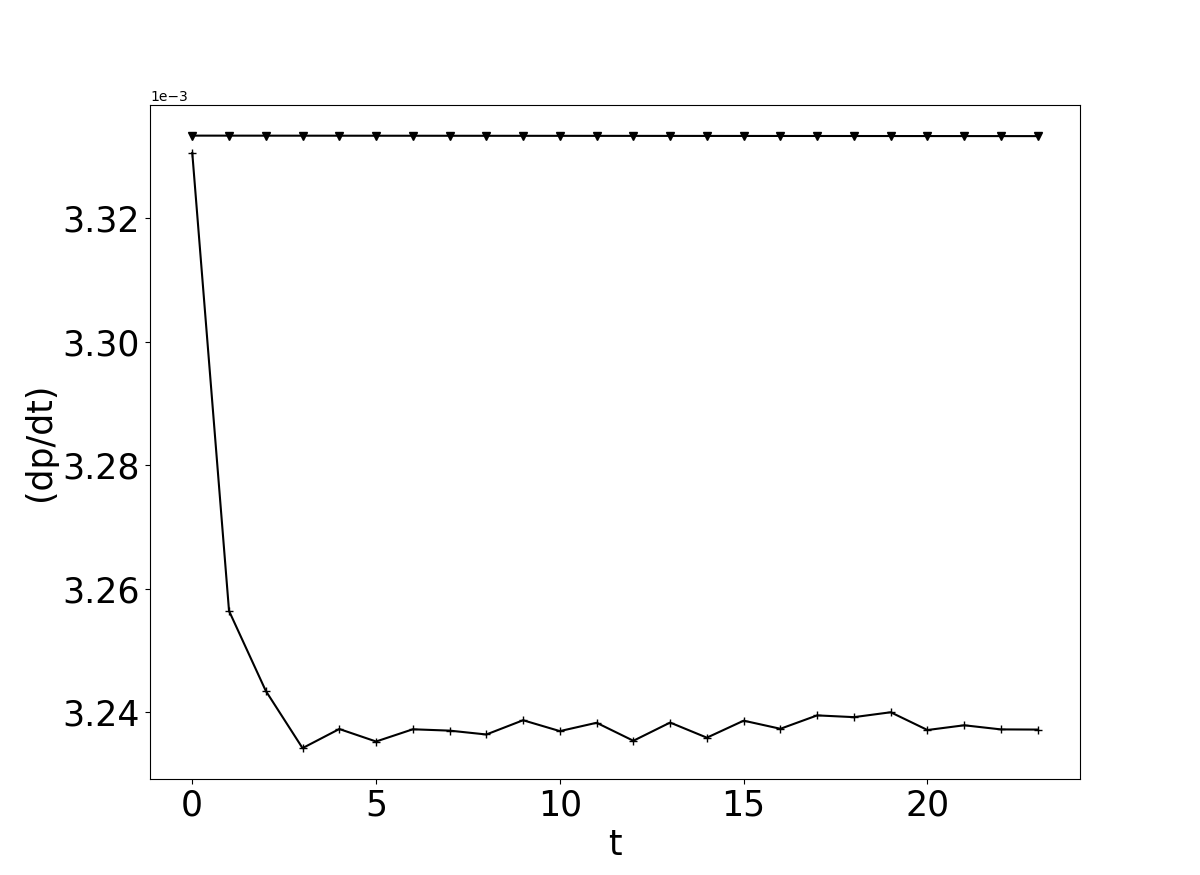
\includegraphics[width=\linewidth]{/home/zachi/Documents/ROM_using_Autoencoders/Bachelorarbeit/Figures/02_12_20/kn0p00001Conservative_Quantities/together/d_dt_p.png}
	\caption{ormalized total change in Energy $\hat{p}$ over time}\label{fig:awesome_image3}
	\endminipage
\end{figure}
\begin{subequations}	
	\begin{align}
	\frac{\frac{d}{dt} \int E \,dx}{\bar{E}} = 0 && &\textrm{with}\quad \bar{E} = \frac{\iint E \,dtdx}{\Delta t}\label{Eq:Con1}\\
	\frac{\frac{d}{dt} \int \rho \,dx}{\bar{\rho}} = 0 && &\textrm{with}\quad \bar{\rho} = \frac{\iint \rho \,dtdx}{\Delta t}\label{Eq:Con2}\\
	\frac{\frac{d}{dt} \int \rho u \,dx}{\bar{\rho u}} = 0 && &\textrm{with}\quad \bar{\rho u} = \frac{\iint \rho u \,dtdx}{\Delta t}\label{Eq:Con3}
	\end{align}
\end{subequations}
\subsubsection{Convolutional Autoncoder}



\subsection{Discussion and Outlook}
\bibliography{Bibliography}{}
\bibliographystyle{unsrt}
\end{document}
